\documentclass[../analysisII_notes.tex]{subfiles}
\begin{document}
\section{Aula 11 - 09 de Abril, 2025}
\subsection{Motivações}
\begin{itemize}
	\item Propriedades da Medida Nula;
	\item Oscilação em um ponto.
\end{itemize}
\subsection{Teorema de Lebesgue}
Estreamos esta aula a partir de exatamente onde paramos anteriormente - a prova das propriedades dos conjuntos de medida nula. Mais especificamente, fora enunciada a proposição
\begin{prop*}[Propriedades dos Conjuntos de Medida Nula]
	\begin{itemize}
		\item[i)] Um conjunto com único ponto é de medida nula:
		      \[
			      m(\{a\}) = 0,\; \forall a\in \mathbb{R};
		      \]
		\item[ii)] Se A e B são subconjuntos da reta real, com A sendo subconjunto de B, então
		      \[
			      m(B) = 0 \Rightarrow m(A) = 0,
		      \]
		      ou seja, um conjunto de medida nula não pode conter um conjunto sem medida nula;
		\item[iii)] Se \((E_{i})_{i\in \mathbb{N}}\) for uma sequência de conjuntos, todos de medida nula, então
		      \[
			      m \biggl(\bigcup_{i=1}^{\infty}E_{i}\biggr) = 0;
		      \]
		\item[iv)] Qualquer intervalo \([a, b]\), com \(a < b\), \textbf{não} tem medida nula.
	\end{itemize}
\end{prop*}
Sem mais delongas,
\begin{proof*}
	(i): para ver que a medida de qualquer conjunto com um único ponto é nula, dado \(\varepsilon \) positivo, considere a cobertura por intervalos fechados
	\[
		\tilde{I}_{n} = \biggl[a - \frac{\varepsilon }{n^{2}}, a+\frac{\varepsilon }{n^{2}}\biggr].
	\]
	De cara, segue que
	\[
		\{a\}\subseteq \bigcup_{n=1}^{\infty} \tilde{I}_{n}.
	\]
	Além disso, para cada \(n\),
	\[
		\ell (I_{n}) = a + \frac{\varepsilon }{n^{2}} - a+\frac{\varepsilon }{n^{2}} = \frac{2\varepsilon }{n^{2}}.
	\]
	Assim,
	\[
		\sum\limits_{n=1}^{\infty}\ell (I_{n}) = \sum\limits_{n=1}^{\infty}\frac{2\varepsilon }{n^{2}} = 2\varepsilon \sum\limits_{j=1}^{n}\frac{1}{n^{2}} = \frac{\varepsilon \pi^{2}}{3}.
	\]
	Com isso, podemos voltar ao início e redefinir a sequência de intervalos para
	\[
		I_{n} =\biggl[a - \frac{3\varepsilon }{(2\pi^{2})n^{2}}, a+\frac{3\varepsilon }{\pi^{2}n^{2}}\biggr],
	\]
	e aqui está a ``beleza'' dos conjuntos de um único ponto - qualquer intervalinho em volta do ponto que compões este conjunto conterá o conjunto todo. Com isto, segue que
	\[
		\sum\limits_{n=1}^{\infty}\ell (I_{n}) = \sum\limits_{n=1}^{\infty}\frac{6\varepsilon }{2\pi^{2}n^{2}} = \frac{6\varepsilon }{2\pi^{2}}\varepsilon \sum\limits_{j=1}^{n}\frac{1}{n^{2}} = \frac{3\varepsilon \pi^{2}}{6\pi^{2}} = \frac{\varepsilon }{2} < \varepsilon.
	\]
	Portanto,
	\[
		m(\{a\}) = 0.
	\]

	ii.) Uma forma semântica de provar este item é: tendo em mente que a medida pode ser pensada metaforicamente como a quantidade de ``conteúdo'' de um conjunto, então é natural pensar que, se um conjunto não tem nada de conteúdo, a única coisa dentro dele é justamente nada de conteúdo; então, qualquer subconjunto dele deve ter nada como conteúdo, significando a medida nula.

	Ficar repetindo isso, além de ser um bom jogo de palavras, ajuda a ilustrar a ideia da prova - iremos, a partir do conjunto maior B, nos restringir à análise do conteúdo do seu subconjunto, e concluir que ela deve ser nula. Na matemática, qual operação fundamental de conjuntos corresponde à restrição de um conjunto a outro dentro dele? A intersecção!

	Com isso, dado \(\varepsilon \) positivo e a cobertura
	\[
		I_{n}:\: B\subseteq \bigcup_{n=1}^{\infty}I_{n},\: \sum\limits_{n=1}^{\infty}\ell (I_{n})<\varepsilon ,
	\]
	considere a cobertura do subconjunto A dada justamente pela restrição de cada \(I_{n}\) ao A:
	\[
		J_{n}\coloneqq I_{n}\cap A.
	\]
	Como, para todo n natural,
	\[
		I_{n}\cap A \subseteq I_{n},
	\]
	vale que os comprimentos satisfazem a relação
	\[
		\ell (J_{n})=\ell (I_{n}\cap A)\leq \ell (I_{n}).
	\]

	Logo, encontramos uma sequência de intervalos tal que, para cada \(\varepsilon \) positivo,
	\[
		B\cap A = A \subseteq \bigcup_{n=1}^{\infty}I_{n}\cap A = \bigcup_{n=1}^{\infty}J_{n}
	\]
	e
	\[
		\sum\limits_{n=1}^{\infty}\ell (J_{n})\leq \sum\limits_{n=1}^{\infty}\ell (I_{n})<\varepsilon .
	\]
	Portanto, \(A\) tem medida nula porque \(B\), que o contém, também possui.

	iii.) A analogia do conteúdo também serve para ilustrar a prova desse item - se eu agrupo um monte de coisa com conteúdo vazio de forma natural, não tem como o resultado criar conteúdo do nada, então, ao final, o conteúdo total ainda será nulo.

	Com base nisso, a ideia por trás dessa prova seria justamente criar uma cobertura para a união dos conjuntos de medida nula que tenha um tamanho tão pequeno quanto desejarmos. Vamos fazer um processo de indução na quantidade de conjuntos de medida nula. Começando pelo caso base, se \(E_1\) e \(E_2\) são tais conjuntos, então existem coberturas
	\[
		I_{i} \quad\&\quad J_{i}
	\]
	de cada um deles, tais que
	\[
		E_1 \subseteq \bigcup_{i=1}^{\infty}I_{i} \quad\&\quad E_2 \subseteq \bigcup_{i=1}^{\infty}J_{i} \Rightarrow E_{1}\cup E_{2}\subseteq \bigcup_{i=1}^{\infty}(I_{i}\cup J_{i}),
	\]
	donde tiramos nossa sequência de intervalos fechados candidata como \(\{I_{n}\cup J_{n}\}\). Sabemos, também, que
	\[
		\sum\limits_{n=1}^{\infty}\ell (I_{n}) < \varepsilon _1 \quad\&\quad \sum\limits_{n=1}^{\infty}\ell (J_{n}) <\varepsilon_{2}.
	\]
	Assim, tomando \(\varepsilon = \frac{1}{2}\max_{}\{\varepsilon_1, \varepsilon_2\},\) vale
	\[
		\sum\limits_{n=1}^{\infty}\ell (I_{n}\cup J_{n}) \leq \sum\limits_{n=1}^{\infty}\ell (I_{n}) + \sum\limits_{n=1}^{\infty}\ell (J_{n}) < \varepsilon +\varepsilon = \max_{}\{\varepsilon_1, \varepsilon_2\},
	\]
	provando o caso base. A partir dele, suponha que, dados \(E_1,\dotsc , E_{n}\) conjuntos de medida nula, a união
	\[
		\bigcup_{i=1}^{n}E_{i}
	\]
	também é de medida nula. Considere, também, \(E_{n+1}\) um conjunto extra de medida nula; nosso objetivo será mostrar que
	\[
		\bigcup_{i=1}^{n}E_{i}\cup E_{n+1}
	\]
	é um conjunto de medida nula. Para isso, denote por
	\[
		\{I_{m_{k}}\}_{1\leq m\leq n}
	\]
	a sequência de intervalos fechados que cobrem o m-ésimo conjunto da sequência original, ou seja, \(\{I_{m_{k}}\}_{k\in \mathbb{N}}\) é uma cobertura para \(E_{m}\). Ademais, sabemos que existe uma sequência
	\[
		\{I_{(n+1)_{k}}\}_{k\in \mathbb{N}}
	\]
	de conjuntos fechados cobrindo \(E_{n+1}\), já que ele tem medida nula. Logo,
	\[
		\bigcup_{m=1}^{n}E_{m}\subseteq \bigcup_{m=1}^{n+1}\bigcup_{k=1}^{\infty}I_{m_{k}}.
	\]
	Além disso, dado \(\varepsilon > 0\), podemos pôr
	\[
		\varepsilon = \frac{\max_{1\leq m\leq n+1}\{\varepsilon_{m}\}}{(n+1)},
	\]
	em que os \(\varepsilon_{m}\)'s são os \(\varepsilon\)'s de cada membro da coleção \(\{E_1, \dotsc , E_{n+1}\}.\) Com isso,
	\[
		\sum\limits_{k=1}^{\infty}\ell \biggl(\bigcup_{m=1}^{n+1}I_{m_{k}}\biggr) \leq \sum\limits_{m=1}^{n+1}\sum\limits_{k=1}^{\infty}\ell (I_{m_{k}}) < \sum\limits_{m=1}^{n+1}\varepsilon_{m} < (n+1)\varepsilon = \max_{1\leq m\leq n+1}\varepsilon_{m}.
	\]
	Portanto, a união
	\[
		\bigcup_{m=1}^{n+1}E_{m}
	\]
	é um conjunto de medida nula e, por indução, isso vale para união enumerável.

	iv.) Exercício? \qedsymbol
\end{proof*}

Trataremos de estabelecer a caracterização mais precisa de quais funções limitadas são Riemann-integráveis num intervalo \([a, b]\) através do seguinte teorema, a ser provado futuramente:
\hypertarget{lebesgue_theorem}{
	\begin{theorem*}[Teorema de Lebesgue]
		Seja \(f:[a, b]\rightarrow \mathbb{R}\) uma função limitada. Então, f é integrável se, e somente se, o subconjunto do domínio dela constituído pelos seus pontos de descontinuidade, \(D\), tem medida nula.
	\end{theorem*}
}
Antes de provarmos ele, devemos trabalhar com alguns conceitos novos sobre oscilações que aparecerão no meio do caminho:

\begin{def*}
	Seja \(f:[a, b]\rightarrow \mathbb{R}\) uma função limitada. Para cada \(x_{0}\) no intervalo \([a, b]\) e número positivo \(\delta \), definimos a \textbf{oscilação de f num intervalo fechado em torno de }\(x_{0}\) como
	\[
		\Omega (x_{0}; \delta )=\omega(f; [a, b]\cap [x_{0}-\delta , x_{0}+\delta ]) = M_{\varepsilon }-m_{\delta },
	\]
	em que
	\begin{align*}
		 & M_{\delta }=\sup_{}\{f(x):x\in [a, b]\cap [x_{0}-\delta , x_{0}+\delta ]\}               \\
		 & m_{\delta }=\inf_{}\{f(x):x\in [a, b]\cap [x_{0}-\delta , x_{0}+\delta ]\}.\quad \square
	\end{align*}
\end{def*}
Com a capacidade de caracterizar a oscilação em torno de uma vizinhança de um ponto, um processo natural é diminuir ela indefinidamente, usando limites, para olhar ponto-a-ponto a oscilação de uma função, que é a motivação da seguinte definição:

\begin{def*}
	Seja \(f:[a, b]\rightarrow \mathbb{R}\) uma função limitada. Para cada \(x_{0}\) no intervalo \([a, b]\) e número positivo \(\delta \), definimos a \textbf{oscilação de f no ponto}\(x_{0}\) como
	\[
		\omega (f; x_{0})=\omega (x_{0})\coloneqq \lim_{\delta \to 0^{+}}\Omega (x_{0}; \delta )=\inf_{\delta > 0}\Omega (x_{0};\delta ). \quad \square
	\]
\end{def*}

\begin{figure}[H]
	\begin{center}
		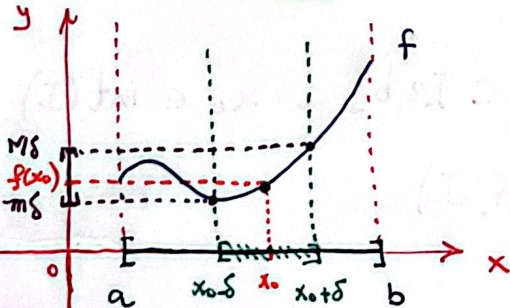
\includegraphics[height=0.4\textheight, width=0.4\textwidth, keepaspectratio]{./Images/around_oscilation_11.png}
	\end{center}
	\caption{ilustração da oscilação em torno de um ponto.}
	\label{arnd11}
\end{figure}
\begin{figure}[H]
	\begin{center}
		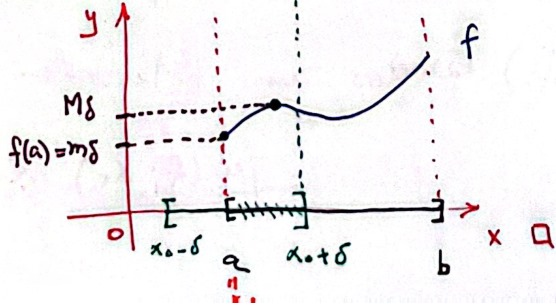
\includegraphics[height=0.4\textheight, width=0.4\textwidth, keepaspectratio]{./Images/point_oscilation_11.png}
	\end{center}
	\caption{ilustração da oscilação em um ponto.}
	\label{at11}
\end{figure}

Para ver que essa definição faz sentido e que a oscilação em um ponto realmente define um número real, precisamos mostrar que aquele ínfimo ao longo de quaisquer \(\delta \)'s faz sentido. Para estes fins, note que, por f ser limitada, \(M_{\delta }\) é maior ou igual a \(m_{\delta }\), o que garante, para todo número positivo \(\delta \), que
\[
	\Omega (x_{0}; \delta )\geq 0 \quad\&\quad \Omega (x_{0}; \delta )\in \mathbb{R}.
\]
Além disso, se \(\delta_{1} < \delta_{2}\), então
\[
	\left\{\begin{array}{ll}
		M_{\delta_{1}}\leq M_{\delta_2} \\
		m_{\delta_{2}}\leq m_{\delta_1}
	\end{array}\right. \Rightarrow \left\{\begin{array}{ll}
		M_{\delta_{1}}\leq M_{\delta_2} \\
		-m_{\delta_{1}}\leq - m_{\delta_2}
	\end{array}\right.
\]
Assim, olhar para \(\Omega \) em função de \(\delta \), ou seja, \(\Omega (x_{0}; \cdot ):(0, \infty)\rightarrow \mathbb{R} \), mostra que ela é não decrescente e que decresce quando \(\delta \) decresce, pois
\[
	\Omega (x_{0}; \delta_{1}) = M_{\delta_{1}} - m_{\delta_{1}} \leq M_{\delta_{2}} - m_{\delta_{2}} = \Omega(x_{0}; \delta_{2}),
\]
o que, junto ao fato de ser uma função limitada inferiormente por 0, garante a existência do ínfimo que define \(\omega(f; x_{0})\), sua não negatividade e a coincidência com o limite à direita.
\end{document}
